\myChapter{État de l’art sur la composition incrémentale des services }{}\label{chap:etat-de-l-art}
%\myMinitoc{Profondeur de la minitoc (section|subsection|subsubsection)}{Titre de la minitoc}
\myMiniToc{mysection}{Sommaire}

% ====section=====
% ====section=====
\mySection{Introduction}{}
% Après avoir posé les bases conceptuelles et techniques liées aux architectures orientées services, aux infrastructures cloud-native et à la transformée de Fourier, ce chapitre a pour objectif d’explorer les travaux existants relatifs à la composition des services, et plus particulièrement à la composition incrémentale.
Après avoir établi les bases conceptuelles et techniques relatives aux architectures orientées services, aux infrastructures cloud-native et à la transformée de Fourier, ce chapitre explore l'évolution des approches de composition de services, depuis les modèles traditionnels vers les paradigmes incrémentaux.


Nous commencerons par situer cette approche dans l'évolution des modèles de composition, en montrant comment les besoins en flexibilité, en scalabilité et en réactivité dans les systèmes modernes ont conduit à dépasser les paradigmes traditionnels. Ensuite, nous présenterons les principes fondamentaux de la composition incrémentale : exécution pilotée par les données, granularité des traitements, activation paresseuse et suivi dynamique des dépendances.

% Nous introduirons ensuite le modèle des \textbf{GAG}, qui constitue une base formelle rigoureuse pour exprimer la logique de composition incrémentale dans un environnement distribué. Ce modèle, fondé sur une extension des grammaires attribuées classiques, permet de représenter la structure et les dépendances entre services tout en assurant une exécution locale et partielle.

Enfin, nous passerons en revue les travaux de recherche et prototypes existants qui exploitent ce paradigme, en mettant en évidence leurs apports, leurs limites et les perspectives ouvertes pour des cas d’application concrets comme celui étudié dans ce mémoire.

% %%%%% Draft %%%%%%
% Après avoir établi les bases conceptuelles et techniques relatives aux architectures orientées services, aux infrastructures cloud-native et à la transformée de Fourier, ce chapitre explore l'évolution des approches de composition de services, depuis les modèles traditionnels vers les paradigmes incrémentaux.

% Dans un premier temps, nous présenterons les fondements techniques des services Web et une taxonomie des approches de composition existantes. Puis, nous détaillerons les principes du calcul incrémental et de l'exécution paresseuse, avant d'examiner les travaux de recherche qui exploitent ces paradigmes. Enfin, nous positionnerons ces approches par rapport aux besoins spécifiques de performance et de réactivité dans les systèmes distribués modernes.
% %%%%% Draft %%%%%%

% ====section=====
% ====section===== 
% \mySection{Origine des Architectures logicielles distribuées}{}
\mySection{Description des Services Web}{}
Les efforts de recherche et de développement récents autour des services Web ont conduit à un certain nombre de spécifications qui définissent aujourd’hui les architectures de référence des services Web. Pour garantir l’interopérabilité dans une SOA, des propositions de standards ont été élaborées. Nous citons, notamment les standards émergents SOAP, WSDL, UDDI et REST.
\begin{itemize}
    \item \textbf{SOAP}: est un protocole de messagerie créé en 1998 pour l'implémentation de services Web \cite{soni2019api}. Il facilite la communication entre applications et les appels RPC en utilisant des messages XML structurés dans des enveloppes SOAP. Ces enveloppes contiennent un en-tête optionnel pour les métadonnées (authentification, routage) et un corps obligatoire pour les données principales. SOAP s'appuie sur les protocoles de transport existants comme HTTP et SMTP plutôt que de créer son propre protocole de communication;
    \item \textbf{WSDL} est  un standard utilisé pour décrire les services SOAP de manière indépendante de leur implémentation. Il définit l'interface du service en séparant la description abstraite de la fonctionnalité des détails concrets d'accès. La partie abstraite décrit le service à travers les messages échangés et inclut des éléments "\textit{operation}" regroupés dans un élément "\textit{interface}", sans spécifier le protocole. La partie concrète établit la liaison entre la définition d'interface et un protocole spécifique. WSDL fournit ainsi tous les détails nécessaires pour localiser le service et comprendre l'ensemble des opérations qu'il prend en charge;
    \item \textbf{UDDI} est un système de registres centralisés qui facilite la découverte des services Web en fonctionnant comme un annuaire numérique \cite{uddi2004v3}. Il organise les informations en trois catégories : pages blanches (noms et contacts), pages jaunes (catégorisation par types de services), et pages vertes (détails techniques). UDDI permet aux utilisateurs de rechercher et localiser systématiquement des fournisseurs de services Web selon leurs caractéristiques spécifiques.
    \item \textbf{REST} est un style architectural basé sur le concept de ressources identifiées par des URI et manipulées via une interface uniforme utilisant les verbes HTTP (\textit{GET, POST, PUT, DELETE}) \cite{soni2019api}. Il s'appuie sur HTTP comme protocole de transport et n'impose aucun format d'échange spécifique, permettant l'utilisation de XML, JSON ou autres formats. Les applications respectant pleinement ces critères sont appelées \textit{RESTful} et permettent de développer des architectures orientées ressources.
\end{itemize}

% \subsection{Évolution des architectures:  monolithique → SOA → microservices}{}
% \subsection{Évolution des architectures}{}
% Cette évolution montre comment les applications sont passées d’un modèle centralisé à une organisation modulaire et distribuée, favorisant l’évolutivité et la réutilisation.

% \subsection{Importance de la modularité et de la réutilisabilité des services}{}
% La modularité permet une maintenance facilitée, la réutilisabilité accélère les cycles de développement et favorise l’intégration de services indépendants dans des systèmes complexes.

% % ====section=====
% \mySection{Apparition des conteneurs et de l’orchestration}{}
% Cette section introduit les technologies qui facilitent le déploiement, la portabilité et la résilience des services dans les environnements cloud-native.

% \subsection{Docker et son rôle dans la portabilité}{}
% Docker permet d'encapsuler des services dans des conteneurs légers et portables, simplifiant leur exécution dans divers environnements sans modification du code.

% \subsection{Kubernetes pour l’orchestration et la résilience des déploiements}{}
% Kubernetes automatise le déploiement, l'équilibrage de charge et la reprise sur panne des conteneurs, garantissant robustesse et scalabilité des services.

% ====section=====
% \mySection{Travaux sur la composition de services}{}
\mySection{Taxonomie sur la composition de services}{}
La composition des services est un concept central dans les architectures orientées services (SOA), qui permet de combiner des services distincts pour créer des applications ou des processus plus complexes. Dans un monde où l'agilité, la réutilisabilité et l'interopérabilité sont des enjeux majeurs, la capacité à assembler efficacement des services devient essentielle. Cependant, cette composition n'est pas un processus unifié, mais se décline en plusieurs approches et stratégies, souvent influencées par les objectifs techniques, les contraintes métier, ou même les évolutions des services eux-mêmes.

%%%%%%%%%%%%% Copy %%%%%%%%%%%%%%%%
\textbf{Composition statique des services}


\textbf{Orchestration.}
L'orchestration des services s'appuie sur divers langages de définition. Cette section détaille les langages les plus employés dans ce domaine :
\begin{itemize}
    \item \textbf{XLANG} est une extension WSDL développée par Microsoft, qui offre un framework d'orchestration de services web et de définition d'accords collaboratifs, basé sur des fondements théoriques de calcul. Les actions constituent ses éléments fondamentaux, intégrant les quatre opérations WSDL standard (requête/réponse, sollicitation, notification) et ajoutant deux catégories spécifiques: \textit{arrêts} (date-limite et durée) et \textit{exceptions};
    \item \textbf{WSFL} Web Services Flow Language \cite{leymann2001web} constitue un langage XML destiné à spécifier les services web composites. Il distingue deux approches compositionnelles : premièrement, la modélisation d'usage coordonné d'un ensemble de services web pour atteindre un objectif métier spécifique, générant ainsi une spécification de processus d'affaires ; deuxièmement, la définition des patterns d'interaction entre services web, produisant une description des échanges globaux associés;
    \item \textbf{BPEL4WS} \cite{juric2006business} (également désigné BPEL ou BPELWS) constitue un langage XML spécialisé dans la spécification des processus d'affaires. Son architecture permet l'échange et la modification de données distribuées entre organismes multiples via l'orchestration de services web. Ce langage modélise les interactions de processus métier fondés sur les services web, tant en contexte intra-entreprise qu'inter-organisationnel. Les organisations adoptant BPEL peuvent établir leurs workflows métier tout en assurant l'interopérabilité à l'échelle corporative et avec leurs partenaires commerciaux dans un écosystème de services web. La spécification BPEL unifie et supplante les standards WSFL et XLANG.  
\end{itemize}

\textbf{Chorégraphie.}
Contrairement à l'orchestration centralisée, la chorégraphie adopte une stratégie décentralisée et coopérative pour assembler les services. Les langages de chorégraphie majeurs comprennent :
\begin{itemize}
    \item \textbf{WSCL} \cite{banerji2002web}: propose une description XML des services web centrée sur leurs échanges conversationnels et la prise en compte des messages transmis. Conçu pour un déploiement complémentaire avec WSDL, WSCL exploite les définitions WSDL pour spécifier les opérations disponibles et leur chorégraphie, tandis que WSDL fournit les implémentations concrètes des définitions de messages et les spécifications techniques des éléments manipulés;
    \item \textbf{WSCI} \cite{w3c2002wsci}: constitue un langage XML axé sur la modélisation des services web comme interfaces définissant les flux de messages échangés (chorégraphie des messages). Il vise à caractériser le comportement externe observable des services en exprimant les dépendances logiques et temporelles inter-messages via des mécanismes de contrôle séquentiel, de corrélation, de gestion d'erreurs et de transactions. WSCI réutilise les définitions abstraites WSDL pour spécifier ultérieurement les modalités d'implémentation concrète des éléments manipulés dans la modélisation de sevices.  
\end{itemize}
 
\textbf{Composition dynamique}

\textbf{Approches orientées Intelligence Artificielle.}
Un service web peut être spécifié à l'aide de ses conditions et effet qui sont des concepts très proches de ceux de la planification.

Plusieurs branches de l'IA intègrent le processus de composition; nous notons notamment:
\begin{itemize}
    \item \textbf{Composition à base de règles}: cette approche de planification s'appuie sur un ensemble de règles prédéfinies et de conditions dans la même philosophie que les déclarations \textit{if-then-else};
    \item \textbf{Composition avec SMA} \cite{kumar2008framework}:  l'implémentation de la composition de services peut exploiter les SMA. Chaque agent représente un service et traite une portion de la requête utilisateur selon ses capacités spécifiques;
    \item \textbf{Calcul situationnel}: cette méthode modélise les requêtes utilisateur et contraintes de services sous forme de prédicats du premier ordre dans le langage de calcul situationnel. Les services sont formalisés comme actions (primitives ou complexes) dans ce même langage. Des modèles sont ensuite générés via des règles de déduction et contraintes, puis instanciés à l'exécution selon les préférences utilisateur; 
    \item \textbf{Composition par planification} \cite{peer2004pddl}:cette approche organise les services web selon leurs préconditions et effets. Diverses méthodes ont été développées pour traiter la composition servicielle comme un problème de planification, notamment l'approche PDDL qui vise à standardiser les données d'entrée des planificateurs. Ce langage propose un formalisme unifié pour décrire les domaines de planification, incitant ainsi la communauté de recherche en services web à l'adapter au contexte compositionnel. 
\end{itemize}

\textbf{Approches Formelles.}
Le modèles sémantiques formels apparaissent comme l'une des meilleures solutions pour spécifier la composition des services web.

Plusieurs formalismes ont été développés dans cette perspective, incluant les automates, diagrammes d'activités, algèbres de processus et réseaux de Pétri.
\begin{itemize}
    \item \textbf{Automate} ces modèles constituent des outils largement employés pour la spécification formelle de systèmes complexes. Un automate comprend un ensemble de nœuds représentant les états et des arcs étiquetés décrivant les transitions inter-états. Dans le contexte de la modélisation compositionnelle de services, chaque appel de service correspond à un état spécifique, un état distinct signale la terminaison d'exécution du service, et chaque réponse génère un événement associé;
    \item \textbf{Diagrammes UML} \cite{jacobson2021unified} UML constitue désormais un standard reconnu pour la modélisation orientée objet de systèmes complexes. Les diagrammes UML se répartissent en trois catégories:(\textit{i}) diagrammes structurels modélisant les aspects statiques (diagrammes de \textit{classes}, d'\textit{objets}), (\textit{ii}) diagrammes comportementaux (diagrammes d'\textit{activités}, d'\textit{états-transitions}), et (\textit{iii}) les diagrammes d'interactions dynamiques (les diagrammes de \textit{séquences}). Le \textit{diagramme d'activité} s'avère particulièrement prisé pour la composition de services web. Dans cette approche, l'exécution de services est généralement représentée par une action, la transition entrante modélise l'invocation du service tandis que la transition sortante signale la fin d'exécution;
    \item \textbf{Algèbre de Processus} \cite{lucchi2007pi} ces familles de langages formels permettent la modélisation de systèmes complexes, notamment les architectures distribuées et concurrentielles; 
    \item \textbf{Réseaux de Pétri} \cite{cheng2014automatic} les RdPs les RdPs constituent un outil de modélisation pour les systèmes dynamiques à événements discrets. Leur principal atout réside dans leur représentation graphique facilitant considérablement la modélisation conceptuelle de systèmes variés. Les RdPs jouissent d'une forte reconnaissance dans le domaine de la gestion des processus métiers (BPM) grâce à leur capacité à modéliser une grande diversité de processus et de flux de contrôle.
\end{itemize}
\begin{figure}[h]
    \centering
    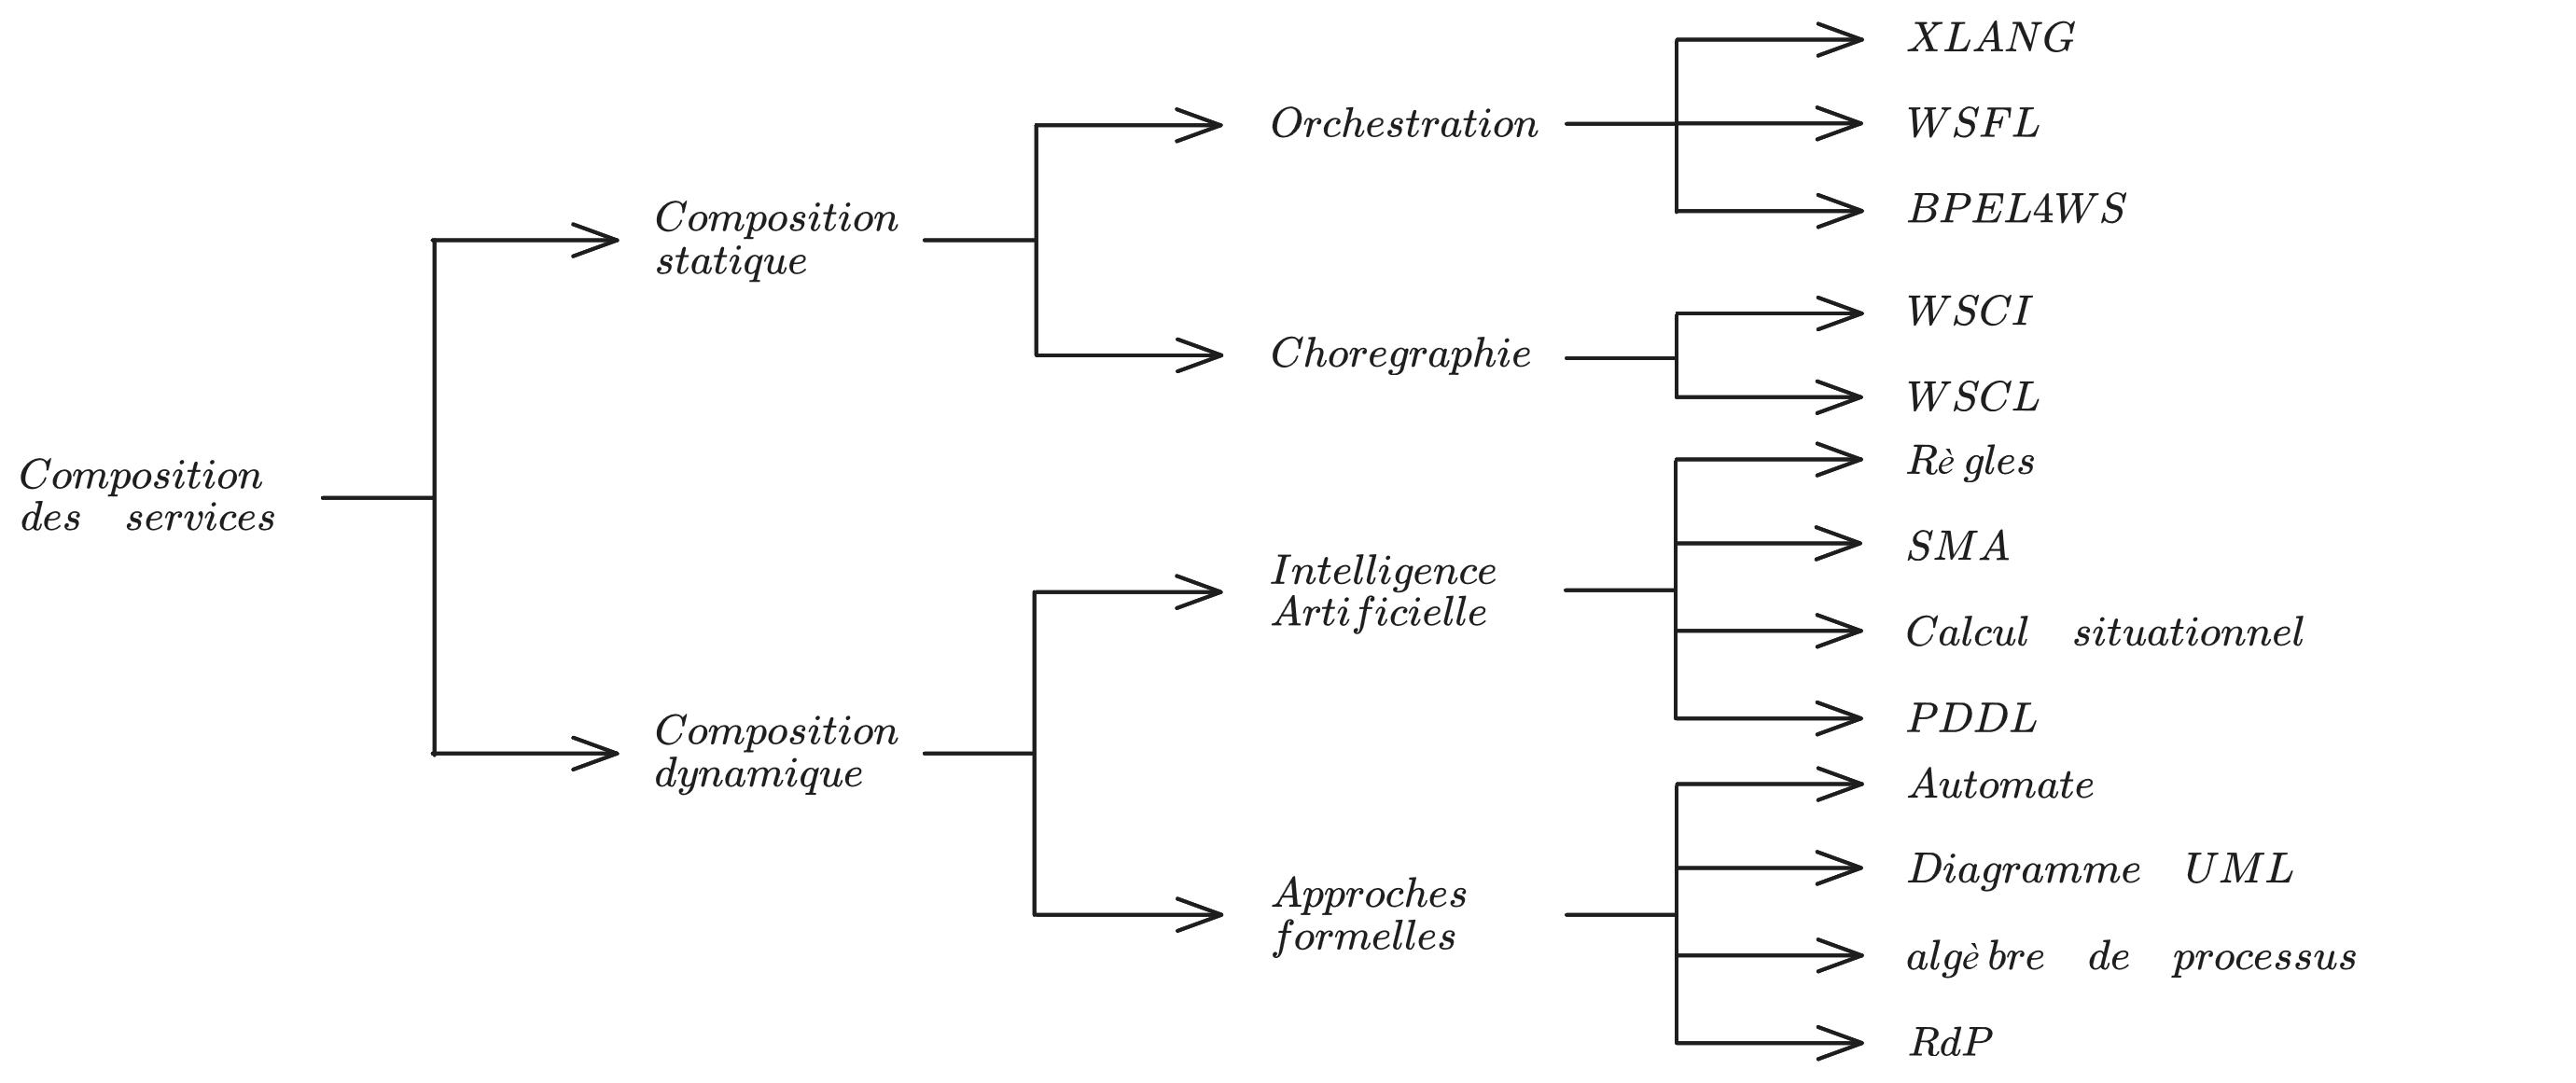
\includegraphics[width=\linewidth]{My-Thesis/Chap2/images/taxonomie des approches de composition des services.png}
    \caption{Taxonomie des approches de composition des services}
    \label{fig:taxonomie-composition}
\end{figure}
La figure \ref{fig:taxonomie-composition} présente une taxonomie hiérarchique de la composition de services structurée en deux approches principales : la composition statique et la composition dynamique. La composition statique se subdivise en orchestration (coordination centralisée utilisant XLANG, WSFL, BPELAWS) et chorégraphie (coordination décentralisée avec WSCI, WSCL), offrant des processus prédéfinis et stables. La composition dynamique comprend les approches d'intelligence artificielle (règles, SMA, calcul situationnel, PDDL) et les approches formelles (automates, diagrammes UML, algèbre de processus, RdP), permettant une adaptation en temps réel. Cette classification illustre l'évolution des paradigmes de composition depuis les approches statiques traditionnelles vers des solutions dynamiques plus flexibles, chaque catégorie répondant à des besoins spécifiques en termes de prévisibilité, contrôle, adaptabilité et vérification formelle dans les architectures orientées services.
%%%%%%%%%%%%% Copy %%%%%%%%%%%%%%%%
% \subsection{Composition Statique vs Dynamique}{}
% La composition statique est rigide et définie à l’avance, alors que la dynamique offre une flexibilité d’exécution selon les contextes et les événements.

% \subsection{Introduction de la composition incrémentale et des modèles de coordination}{}
% La composition paresseuse permet de retarder l’exécution des services jusqu’à ce que leurs données soient disponibles, optimisant ainsi les ressources.

% ====section=====
\mySection{Calcul incrémental et exécution paresseuse}{}
Dans les environnements modernes, où les services sont hautement distribués et les données souvent partielles ou disponibles de façon asynchrone, il devient indispensable de concevoir des mécanismes de composition qui s’adaptent dynamiquement à l’état du système. Contrairement aux modèles traditionnels, qui supposent une orchestration globale et rigide, le calcul incrémental et l’exécution paresseuse offrent une alternative plus souple, réactive et localement autonome. Ces paradigmes permettent de déclencher uniquement les services nécessaires, au moment où leurs dépendances sont satisfaites, réduisant ainsi la consommation de ressources tout en augmentant la résilience et la scalabilité.

\subsection{Les GAG pour la collaboration distribuée}{}
\label{awgag}
Éric Badouel et al. \cite{badouel2015active} ont proposé dans leur article \textit{"Active Workspaces: Distributed Collaborative Systems based on Guarded Attribute Grammars"} %un formalisme novateur appelé \textbf{Grammaires Attribuées Gardées (GAG)}, destiné à modéliser des systèmes collaboratifs distribués. Leur objectif est de permettre une exécution locale et partielle des processus, en fonction de la disponibilité effective des données.
une nouvelle approche pour la conception de systèmes collaboratifs distribués, en introduisant le modèle des Active Workspaces (AW), combiné au formalisme des Grammaires Attribuées Gardées (GAG). Le contexte de cette contribution est celui des systèmes de gestion de processus métier, traditionnellement fondés sur des modèles de workflow centralisés. Ces derniers orchestrent les tâches à accomplir mais présentent plusieurs limitations majeures : les données sont souvent négligées dans la logique du processus, et les parties prenantes humaines sont considérées comme de simples ressources passives. De plus, la rigidité et la centralisation de ces modèles les rendent peu adaptés à des environnements dynamiques et distribués.

Pour remédier à cela, les auteurs s’appuient sur le concept d’espace de travail actif (AW), une évolution des cartes mentales, qui permet à chaque utilisateur d’organiser ses tâches et de collaborer de manière asynchrone avec d’autres. Le problème que l’article adresse est donc celui de la modélisation cohérente et distribuée de la collaboration, sans orchestration centrale, en intégrant à la fois la structure des données, les règles de transformation, et la participation active des utilisateurs.

\textbf{Méthodologie.}
Les auteurs ont définit un Active Workspace comme un arbre structuré personnel à chaque utilisateur, représentant ses tâches, enrichi par des attributs de données qui guident l’exécution. Ce modèle s’inspire des cartes mentales, avec une orientation vers l’interactivité et la collaboration distribuée.

Les GAG sont utilisées pour formaliser les transformations de l’arbre : chaque règle de production exprime comment une tâche (nœud) peut être décomposée en sous-tâches, sous conditions de garde (conditions sur les données disponibles).

L’exécution est répartie entre les utilisateurs. Chacun dispose d’une vue locale de l’artefact partagé et peut appliquer des règles de manière autonome, sans coordination centrale, dès que les données locales satisfont les conditions.

Les changements locaux sont diffusés via un système de messagerie asynchrone. Lorsqu’un utilisateur modifie un nœud, ses effets sont propagés aux autres parties concernées du système, assurant une cohérence distribuée entre les workspaces.

Plutôt que d’orchestrer les tâches à l’aide d’un moteur central, les auteurs ont laissé aux GAG le soin d’implementer implicitement la coordination, en encodant dans les gardes les conditions nécessaires pour que les règles soient applicables. Ainsi, la progression des tâches s’adapte naturellement à l’état courant des données.

% Les auteurs remplacent l’orchestration centralisée par une coordination implicite, rendue possible grâce aux gardes dans les GAG, qui déterminent localement quand une tâche peut progresser. La logique d’exécution s’ajuste ainsi automatiquement à l’état des données disponibles.

\textbf{Résultats.}
Pour évaluer leur approche, les auteurs ont illustré leur modèle à travers un système de surveillance des maladies. Ce cas pratique consiste en un processus distribué où plusieurs acteurs, tels que des médecins, des biologistes, et des épidémiologistes, collaborent pour suivre et analyser des cas suspects de maladies infectieuses.

Dans ce contexte, chaque acteur, dispose d’un espace de travail actif représenté par une carte structurée en arbre, où chaque nœud correspond à une tâche ou une information (figure \ref{fig:aw-clinicien}). Lorsqu'une tâche doit être effectuée, un nœud ouvert est créé, décrivant le travail à faire. La communication entre acteurs se fait par messages asynchrones, permettant une gestion distribuée.
Ce modèle permet de décomposer le processus, d’assurer l’automatisation des transferts d’informations, et de garantir la flexibilité du système. Il montre que la modélisation par GAG facilite la coordination distribuée tout en conservant modularité, cohérence et adaptabilité.

\begin{figure}[h]
    \centering
    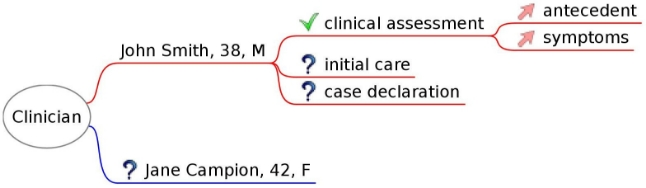
\includegraphics[width=0.7\linewidth]{My-Thesis/Chap2/images/workspace clinicien.png}
    \caption{Espace de travail actif d'un clinicien \cite{badouel2015active}}
    \label{fig:aw-clinicien}
\end{figure}

%chaque utilisateur dispose d’un espace de travail actif représenté par une carte mentale structurée en arbre. Chaque nœud de cet arbre correspond à une tâche ou une information en cours de traitement, par exemple, la déclaration d’un cas, l’envoi d’échantillons, ou l’analyse des résultats. Lorsqu’un utilisateur doit effectuer une tâche, celui-ci active un nœud ouvert, qui définit la nature du travail à faire et le contexte associé. La communication et la coordination entre les acteurs se font par échange de messages asynchrones, ce qui permet une distribution efficace du processus sans besoin de mémoire partagée.

% L’approche utilisant les GAG permet, dans ce cas, de modéliser la décomposition hiérarchique du processus, la gestion des tâches en parallèle, et la transmission automatique des informations entre parties prenantes. De plus, les règles métier intégrées dans le modèle assurent que chaque étape respecte la logique définie, tout en laissant une grande souplesse dans l’organisation des activités. Cela a montré que leur modèle permet non seulement de représenter précisément un processus distribué complexe, mais aussi de garantir sa flexibilité et sa modularité en temps réel.

En résumé, leur solution a permis de simuler un processus collaboratif multi-acteurs où chaque partie peut évoluer indépendamment, tout en étant cohérente avec l’ensemble grâce aux règles formelles. Cela a démontré que la modélisation par GAG est adaptée pour gérer efficacement des systèmes collaboratifs distribués, flexibles et réactifs, permettant une meilleure coordination dans des environnements décentralisés et potentiellement dégradés.

\subsection{Processus d'entreprises distribués et disponibles via GAG et Publish/Subscribe}
\label{pub/sub-rs}
Maurice Tchoupé et Joskel Tagueu \cite{tchendji2021guarded} ont proposé dans leur article \textit{"Guarded Attribute Grammars and Publish/Subscribe for implementing distributed collaborative business processes with high data availability"} un système collaboratif distribué utilisant des Grammaires Attribuées Gardées (GAG) et un protocole de \text{publish/subscribe avec redirection de souscriptions (PubSub-RS)} pour améliorer la disponibilité des données et faciliter la communication asynchrone entre les acteurs, améliorant ainsi la collaboration dans les processus métier sur différents sites géographiques. 

\textbf{Méthodologie.}
La méthodologie proposée dans l'article se divise en plusieurs étapes clés pour implémenter des processus métiers distribués utilisant GAG et le protocole pub/sub-RS. Tout d’abord, à partir d’une description textuelle du processus, les acteurs sont identifiés, et leurs GAG locaux sont spécifiés. Ensuite, un moteur GAG est développé pour exécuter ces processus en environnement distribué. La communication entre acteurs s’appuie sur le protocole pub/sub-RS, qui assure la transmission incrémentale et en temps réel des données semi-structurées, même partiellement produites, par le biais de la redirection des souscriptions.

Une architecture basée sur des composants est également proposée pour déployer ces processus, permettant une exécution distribuée efficace et flexible. La méthodologie inclut ainsi la formalisation des processus, la mise en œuvre des GAG locaux, le développement d’un moteur d’exécution, et la configuration d’un système de communication pub/sub-RS permettant la synchronisation et la collaboration entre acteurs en temps réel. % Cette approche a été expérimentée via un prototype dans le cadre d’un processus de gestion de soumission de thèses, illustrant sa faisabilité et ses avantages en termes de disponibilité et de collaboration.

\textbf{Résultats.}
Pour évaluer leur approche, les auteurs ont illustré leur solution à travers le processus de soumission de thèse à l’université de Dschang. Dans ce contexte, plusieurs acteurs, tels que l’étudiant, le département, l’école doctorale et le rectorat, participent de manière distribuée à différentes étapes du traitement du dossier. La solution modélisée avec GAG et communiquant via le protocole pub/sub-RS permet de suivre en temps réel chaque étape du processus. Lorsqu’une étape est effectuée, comme l’approbation par le rectorat, l’information est immédiatement transmise à tous les acteurs concernés, même si les données sont produites de façon collaborative et incrémentale par plusieurs acteurs. Cette capacité assure que chaque acteur, en particulier l’étudiant, est rapidement informé des avancées ou des rejets de son dossier, facilitant une gestion plus dynamique et une prise de décision plus rapide tout au long du processus. Ces résultats montrent que l’approche permet d’assurer une haute disponibilité et une synchronisation efficace des données dans un contexte distribué et collaboratif.

\subsection{Vers une exécution incrémentale dans les architectures orientées services}{}

\subsubsection{Architecture orientée services basée sur les calculs incrémentaux}
\label{lazy-services}
% Joskel Tagueu et al. \cite{tagueu2021lazy} ont mis sur pied les \textbf{services paresseux}, qui permettent de consommer des données et de produire des résultats de manière incrémentielle, améliorant ainsi l'architecture orientée services (SOA) en favorisant le couplage faible et en optimisant la gestion des abonnements pour les implémentations distribuées, améliorant ainsi l'interopérabilité et l'efficacité des systèmes complexes.
Joskel Tagueu et al. \cite{tagueu2021lazy} ont proposé dans leur article \textit{"Lazy Services: A Service Oriented Architecture based on Incremental Computations and Commitments"} une architecture orientée services novatrice basée sur le calcul incrémental et le concept de \textbf{services paresseux}. Leur objectif est de répondre aux limites des modèles classiques de composition de services, en proposant une exécution réactive, progressive et pilotée par les données, adaptée aux environnements distribués dynamiques.
Les systèmes orientés services classiques supposent généralement que toutes les données nécessaires à l’exécution d’un service sont disponibles dès son déclenchement (approche \textit{tout ou rien}). Cette hypothèse est difficile à maintenir dans des contextes où les données arrivent progressivement, de manière asynchrone ou partielle — comme c’est souvent le cas dans les environnements cloud-native, les systèmes IoT, ou les workflows scientifiques distribués. L’objectif de l’article est de formaliser une exécution \textit{lazy} (paresseuse), dans laquelle un service est activé au fur et à mesure que ses dépendances sont satisfaites, tout en permettant une production incrémentale de ses résultats.

\textbf{Méthodologie.}
L’architecture proposée repose sur plusieurs concepts clés :
\begin{itemize}
    \item \textbf{Services paresseux :} un service est défini par un ensemble d’engagements sur les données qu’il produira, sans attendre que l’ensemble de ses entrées soit complètement disponible;
    \item \textbf{Utilisation des Grammaires Attribuées Gardées (GAG) :} les services sont formalisés comme des règles de production dont les gardes expriment les conditions d’activation. Ces règles permettent d’exécuter les services partiellement, dès qu’une portion de données est disponible;
    \item \textbf{Propagation incrémentale :} chaque production partielle de données peut déclencher d’autres services en aval, créant ainsi une exécution réactive et distribuée, sans plan d’ordonnancement global;
    \item \textbf{Engagements :} les services publient à l’avance les résultats qu’ils s’engagent à produire, ce qui permet aux services consommateurs de s’organiser sans attendre leur production effective.
\end{itemize}

\textbf{Résultats.}
Les auteurs ont validé leur approche par une expérimentation portant sur des processus de composition de services scientifiques. Le scénario testé montre que :
\begin{itemize}
    \item les services peuvent être déclenchés progressivement et en parallèle dès qu’une partie de leurs dépendances est disponible;
    \item la stratégie paresseuse réduit le temps global d’exécution dans un contexte de données partiellement disponibles;
    \item l’exécution devient naturellement tolérante aux défaillances ponctuelles, car la progression du processus dépend uniquement des données locales disponibles et non d’une orchestration centrale.
\end{itemize}

Cette architecture a montré une capacité élevée à gérer des dépendances complexes et à offrir une meilleure scalabilité dans des environnements distribués.

\subsubsection{Moteur de composition incrémentale}{}
\label{incremental-compputation}
Joskel Tagueu et al. \cite{tagueu2024service} ont présenté dans leur article \textit{"A Service Composition Engine for Incremental Computation"} une architecture orientée services reposant sur un moteur d’exécution distribué basé sur les \textbf{Grammaires Attribuées Gardées (GAG)}. L’objectif de ce moteur est de permettre une exécution réactive, flexible et incrémentale des services dans un environnement cloud-native, en s’appuyant sur des composants conteneurisés et orchestrés par Kubernetes.

\textbf{Contexte et objectif.}
Les architectures modernes exigent des systèmes capables de gérer dynamiquement des services distribués, dont les données peuvent être disponibles de manière partielle ou asynchrone. Les moteurs de composition classiques sont souvent limités par une orchestration rigide et centralisée, qui ne s’adapte pas facilement à la nature dynamique des environnements cloud, edge, ou orientés flux. Le moteur de composition proposé vise à offrir une exécution autonome, résiliente et hautement distribuée, où chaque service est activé localement selon l’état de ses dépendances de données.

\textbf{Méthodologie.}
Le moteur repose sur une infrastructure modulaire, articulée autour de plusieurs technologies :

\begin{itemize}
    \item \textbf{Déclaration des services :} Chaque service est spécifié sous forme d’une règle GAG dans un fichier YAML, décrivant ses entrées, sorties et conditions d’activation;
    
    \item \textbf{Fonctions locales :} Les terminaux (fonctions de traitement) sont codés en Java et associés aux règles de production;
    
    \item \textbf{Conteneurisation :} L’ensemble des composants est embarqué dans des conteneurs Docker. Un compilateur assemble les spécifications, les fonctions Java et un moteur GAG dans un artefact .jar prêt à être exécuté;

    \item \textbf{Déploiement distribué :} Les conteneurs sont orchestrés sur un cluster Kubernetes. Chaque conteneur expose une API REST et communique via des messages asynchrones de type publish/subscribe;

    \item \textbf{Exécution incrémentale :} Le moteur exécute les règles dès que leurs gardes sont satisfaites localement. Chaque production partielle de données peut activer en cascade d’autres services, garantissant une exécution fluide, parallèle et adaptative.
\end{itemize}

Cette méthodologie permet de découpler entièrement la spécification fonctionnelle du service de son déploiement, tout en assurant une exécution pilotée par les données disponibles.

\textbf{Résultats.}
Les auteurs ont validé le fonctionnement du moteur en l’appliquant à l’exécution distribuée de l’algorithme de tri par fusion (merge sort). L’approche démontre plusieurs bénéfices :
\begin{itemize}
    \item \textbf{Parallélisme naturel :} Chaque sous-composant du tri (division et fusion) est traité indépendamment dès que ses données sont disponibles;
    \item \textbf{Réactivité :} L’exécution se déclenche localement sans attendre la disponibilité complète du processus global.
    \item \textbf{Tolérance aux défaillances :} Les services non concernés par une panne continuent à fonctionner, renforçant la robustesse de l’exécution;
    \item \textbf{Interopérabilité cloud-native :} Le moteur est compatible avec Kubernetes, Docker, REST, facilitant l’intégration dans des pipelines DevOps.
\end{itemize}

% \textbf{Limites}
% Le prototype est encore en phase de développement expérimental et la limites majeure identifiée est la 
% \textbf{Scalabilité non testée à grande échelle :} L’expérimentation a été réalisée sur une machine locale ; l’évaluation sur des clusters multi-nœuds reste à faire.

% \begin{itemize}
%     \item \textbf{Scalabilité non testée à grande échelle :} L’expérimentation a été réalisée sur une machine locale ; l’évaluation sur des clusters multi-nœuds reste à faire.
%     % \item \textbf{Configuration manuelle :} Le couplage entre fichiers YAML, classes Java et configuration de déploiement nécessite des manipulations techniques.
%     % \item \textbf{Couplage implicite :} Bien que les services soient autonomes, la logique des dépendances n’est pas encore détectée automatiquement, nécessitant un effort de spécification rigoureux.
% \end{itemize}

% En 2024 Joskel Tagueu et al. \cite{tagueu2024service} ont mis sur pied un moteur de composition incrémentale. % active les services en fonction des dépendances résolues, favorisant le parallélisme et l’adaptation dynamique.

% \textbf{Methodologie}
% La méthodologie adoptée dans cet article repose sur l'utilisation d'un cadre formel basé sur les Grammaires d'Attributs Gardées (GAG) pour la modélisation et la spécification des services distribués. Cette approche permet de décrire de manière déclarative la logique des services, leur communication et leur orchestration. L'article combine cette modélisation avec le développement d’un prototype basé sur Kubernetes, permettant de déployer et gérer automatiquement ces services dans un environnement distribué.

% Plus précisément, la démarche comprend plusieurs étapes clés :
% \begin{enumerate}
%     \item La définition formelle des services à l’aide de GAG, qui spécifient à la fois la logique de calcul et les conditions de déploiement via des règles guarded;
%     \item La mise en œuvre de ces services sous forme de conteneurs, facilitant leur déploiement dans une infrastructure orchestrée par Kubernetes;
%     \item La conception d’un langage déclaratif permettant de programmer la composition, la communication et la gestion des services, tout en supportant la computation incrémentale, grâce à la modélisation des processus sous forme de co-routines;
%     \item La validation du modèle par des expérimentations concrètes, notamment la réalisation d’algorithmes classiques distribués, tels que le tri fusion, pour illustrer la flexibilité et la puissance de cette approche.
% \end{enumerate}

% Ainsi, cette méthodologie combine une base théorique solide avec une mise en œuvre pratique, permettant à la fois la modélisation formelle, le déploiement automatique, et la gestion optimale des ressources dans des environnements distribués.

% \subsection{Discussion}

% L’analyse des contributions présentées précédemment révèle une convergence conceptuelle forte autour de la composition incrémentale comme réponse aux limitations des modèles de composition traditionnels. Cette section discute les apports méthodologiques, les choix technologiques communs et les métriques retenues pour l’évaluation des moteurs de composition.

% \textbf{Approche méthodologique.}  
% Tous les travaux examinés adoptent une démarche incrémentale et pilotée par les données, articulée autour d’un modèle formel — les \textbf{Grammaires Attribuées Gardées (GAG)} — et d’une logique de composition décentralisée. Chaque moteur de composition, qu’il s’agisse du système Active Workspaces, des Lazy Services ou du moteur de composition incrementale, repose sur la même philosophie : activer les services uniquement lorsque leurs dépendances sont satisfaites, sans ordonnanceur centralisé.

% \textbf{Évaluation expérimentale.}  
% Les différents moteurs ont été testés sur des cas concrets (soumission de thèse, tri par fusion), en comparant l’approche incrémentale aux compositions classiques. Ces évaluations s’appuient sur une architecture commune : conteneurisation des services (Docker), orchestration (Kubernetes) et communication asynchrone (Pub/Sub-RS). Comme le montre la figure~\ref{fig:cari_architecture}, les composants sont déployés de manière modulaire et répliquée pour favoriser l’indépendance et la tolérance aux pannes.

\subsection*{Discussion}
La composition incrémentale des services, telle qu’implémentée via les Grammaires Attribuées Gardées (GAG), présente plusieurs avantages notables dans le contexte des architectures orientées services. Tout d’abord, le caractère paresseux de l’évaluation permet de réduire significativement la charge computationnelle en ne recalculant que les sous-arbres affectés par une modification de la requête ou des données d’entrée. Cette granularité fine améliore la réactivité du système, particulièrement dans les scénarios où les données évoluent fréquemment ou de manière asynchrone. 

En outre, l’utilisation d’une approche déclarative sépare clairement la spécification de la composition du code d’exécution, facilitant la maintenabilité et l’extensibilité du moteur de composition. La modularité introduite par la définition de services paresseux permet également de réutiliser des composants au sein de différents pipelines de traitement, contribuant à la cohérence et à la réduction de la duplication de logique métier.

Cependant, cette approche présente également des limites. Le surcoût initial lié à l’instanciation du moteur GAG et à la construction de l’arbre de dépendances peut entraîner une latence plus élevée pour les petites requêtes ponctuelles, par rapport à une composition statique optimisée. De même, la gestion de l’état intermédiaire et la persistance des attributs gardés nécessitent un accompagnement sophistiqué (caches, invalidation fine), sous peine de voir la complexité mémoire s’envoler dans des traitements à large échelle.

Enfin, bien que la GAG offre un formalisme puissant pour exprimer la composition incrémentale, son adoption reste encore limitée dans l’industrie.
En résumé, la composition incrémentale via GAG représente une avancée prometteuse pour les systèmes orientés services à forte dynamique de données, mais sa maturité devra être consolidée par des optimisations du moteur, une meilleure prise en charge de l’environnement distribué et des efforts de standardisation pour convaincre les praticiens de l’adopter.


% Les travaux présentés dans les sections précédentes suivent une évolution logique cohérente, depuis les fondements théoriques jusqu'à l’implémentation logicielle complète d’un moteur de composition incrémentale. Cette section a pour objectif de récapituler les apports de chaque contribution, de mettre en lumière les complémentarités entre les approches, et de souligner les points forts ainsi que les limitations identifiées.

% \textbf{Une progression structurée des concepts.}  
% Les \textbf{Grammaires Attribuées Gardées (GAG)}, introduites en \ref{awgag}, constituent le socle théorique sur lequel repose l’ensemble de l’approche. Elles permettent de formaliser les dépendances de données entre services, et d’exprimer la logique de coordination locale sans recourir à un orchestrateur centralisé. Ce modèle garantit une exécution incrémentale, décentralisée et guidée par la disponibilité des données.

% Dans la section \ref{pub/sub-rs}, ce formalisme a été enrichi par l’intégration du protocole \textbf{Publish/Subscribe à redirection de souscriptions (PubSub-RS)}, permettant la communication asynchrone entre services distribués. Ce couplage entre GAG et Pub/Sub offre une base pratique pour exécuter des processus collaboratifs réactifs et interconnectés.

% Les sections \ref{lazy-services} et \ref{incremental-compputation} prolongent cette base en introduisant le concept de \textbf{services paresseux}, qui consomment et produisent leurs données de manière partielle et progressive. Ces services, définis à partir des GAG et du modèle PubSub, incarnent une approche data-driven de la composition. Le \textbf{moteur de composition incrementale}, présenté en \ref{incremental-compputation}, constitue l’implémentation concrète de cette vision, en intégrant les composants dans des conteneurs Docker orchestrés par Kubernetes. Cela permet de bénéficier à la fois de la flexibilité des GAG et de la robustesse des infrastructures cloud-native.

% \textbf{Une complémentarité forte entre les contributions.}  
% Chacune des contributions aborde un niveau différent de la problématique :
% \begin{itemize}
%     \item les \textbf{GAG} fournissent le modèle formel de coordination incrémentale ;
%     \item le \textbf{protocole PubSub-RS} assure la diffusion asynchrone des données ;
%     \item les \textbf{services paresseux} formalisent l’exécution partielle pilotée par les données ;
%     \item le \textbf{moteur de composition} fournit une infrastructure logicielle concrète et réutilisable.
% \end{itemize}

% Ces couches s’articulent de manière fluide : les GAG définissent les règles, le Pub/Sub assure leur synchronisation, les services paresseux en tirent parti pour mettre en œuvre l’évaluation paresseuse, et le moteur déploie cette logique à grande échelle dans un environnement cloud-compatible.

% \textbf{Limites et pistes d’amélioration.}  
% Malgré les avancées notables, plusieurs limites demeurent :
% \begin{itemize}
%     \item Le protocole PubSub-RS, devrait être évalué à plus grande échelle dans des environnements industriels.
%     \item Le moteur de composition reste encore expérimental, et son évaluation sur des cas d’usage complexes reste à approfondir.
% \end{itemize}

% Ces limites offrent autant d’opportunités de recherche future, notamment en matière d’optimisation des communications, d’assistance à la génération automatique des GAG, ou encore d’intégration avec des architectures serverless.


% ====section=====
% ====section=====
\mySection{Conclusion}{}
% Le panorama des travaux présentés dans ce chapitre met en évidence l’évolution des architectures logicielles distribuées, depuis les approches monolithiques et SOA vers les microservices et l’émergence de la composition incrémentale. Nous avons montré que, face aux limites des compositions statiques et dynamiques classiques, les Grammaires Attribuées Gardées (GAG) offrent un modèle déclaratif et paresseux particulièrement adapté aux systèmes à forte variabilité de données.
% L’étude des principaux modèles a permis de dégager les points forts et faibles de chaque approche, la GAG se démarque par sa séparation claire entre spécification et exécution, ainsi que par sa capacité à ne recalculer que les portions réellement impactées.
% Cependant, ces bénéfices s’accompagnent de défis non négligeables: complexité initiale de mise en œuvre, coûts de synchronisation dans des environnements distribués, et maturité encore limitée côté industrialisation et outils de support. C’est pourquoi la discussion insiste sur la nécessité d’optimiser les moteurs GAG et de renforcer les mécanismes de cohérence et de tolérance aux pannes.
% Ce bilan ouvre naturellement sur le chapitre suivant : la conception et l’évaluation expérimentale d’un benchmark basé sur la transformée de Fourier, qui permettra de quantifier précisément l’impact de la composition incrémentale via GAG sur des cas d’usage concrets.

Le panorama des travaux présentés dans ce chapitre met en évidence l’évolution des architectures logicielles distribuées, depuis les approches monolithiques et SOA vers les microservices et l’émergence de la composition incrémentale. Nous avons montré que, face aux limites des compositions statiques et dynamiques classiques, les Grammaires Attribuées Gardées (GAG) offrent un modèle déclaratif et paresseux particulièrement adapté aux systèmes à forte variabilité de données.
L’étude des principaux modèles a permis de dégager les points forts et faibles de chaque approche, la GAG se démarque par sa séparation claire entre spécification et exécution, ainsi que par sa capacité à ne recalculer que les portions réellement impactées.
Cependant, ces bénéfices s’accompagnent de défis non négligeables: complexité initiale de mise en œuvre, coûts de synchronisation dans des environnements distribués, et maturité encore limitée côté industrialisation et outils de support.
Ce bilan ouvre naturellement sur le chapitre suivant: la conception et l’évaluation expérimentale d’un benchmark basé sur la transformée de Fourier, qui permettra de quantifier précisément l’impact de la composition incrémentale via GAG sur des cas d’usage concrets. 